%!TEX program = xelatex

\documentclass[a4paper, openany, oneside]{memoir}
\usepackage[no-math]{fontspec}
\usepackage{pgfplots}
\pgfplotsset{compat=newest}
\usepackage{commath}
\usepackage{mathtools}
\usepackage{amssymb}
\usepackage{amsthm}
\usepackage{booktabs}
\usepackage{mathtools}
\usepackage{xcolor}
\usepackage[separate-uncertainty=true, per-mode=symbol]{siunitx}
\usepackage[noabbrev, capitalize]{cleveref}
\usepackage{listings}
\usepackage[american inductor, european resistor]{circuitikz}
\usepackage{amsmath}
\usepackage{amsfonts}
\usepackage{ifxetex}
\usepackage[dutch,english]{babel}
\usepackage[backend=bibtexu,texencoding=utf8,bibencoding=utf8,style=ieee,sortlocale=en_GB,language=auto]{biblatex}
\usepackage[strict,autostyle]{csquotes}
\usepackage{parskip}
\usepackage{import}
\usepackage{standalone}
\usepackage{hyperref}
%\usepackage[toc,title,titletoc]{appendix}

\ifxetex{} % Fonts laden in het geval dat je met Xetex compiled
    \usepackage{fontspec}
    \defaultfontfeatures{Ligatures=TeX} % To support LaTeX quoting style
    \setromanfont{Palatino Linotype} % Tover ergens in Font mapje in root.
    \setmonofont{Source Code Pro}
\else % Terug val in standaard pdflatex tool chain. Geen ondersteuning voor OTT fonts
    \usepackage[T1]{fontenc}
    \usepackage[utf8]{inputenc}
\fi
\newcommand{\references}[1]{\begin{flushright}{#1}\end{flushright}}
\renewcommand{\vec}[1]{\boldsymbol{\mathbf{#1}}}
\newcommand{\uvec}[1]{\boldsymbol{\hat{\vec{#1}}}}
\newcommand{\mat}[1]{\boldsymbol{\mathbf{#1}}}
\newcommand{\fasor}[1]{\boldsymbol{\tilde{\vec{#1}}}}
\newcommand{\cmplx}[0]{\mathrm{j}}
\renewcommand{\Re}[0]{\operatorname{Re}}
\newcommand{\Cov}{\operatorname{Cov}}
\newcommand{\Var}{\operatorname{Var}}
\newcommand{\proj}{\operatorname{proj}}
\newcommand{\Perp}{\operatorname{perp}}
\newcommand{\col}{\operatorname{col}}
\newcommand{\rect}{\operatorname{rect}}
\newcommand{\sinc}{\operatorname{sinc}}
\newcommand{\IT}{\operatorname{IT}}
\newcommand{\F}{\mathcal{F}}

\newtheorem{definition}{Definition}
\newtheorem{theorem}{Theorem}


\DeclareSIUnit{\voltampere}{VA} %apparent power
\DeclareSIUnit{\pii}{\ensuremath{\pi}}

\hypersetup{%setup hyperlinks
    colorlinks,
    citecolor=black,
    filecolor=black,
    linkcolor=black,
    urlcolor=black
}

% Example boxes
\usepackage{fancybox}
\usepackage{framed}
\usepackage{adjustbox}
\newenvironment{simpages}%
{\AtBeginEnvironment{itemize}{\parskip=0pt\parsep=0pt\partopsep=0pt}
\def\FrameCommand{\fboxsep=.5\FrameSep\shadowbox}\MakeFramed{\FrameRestore}}%
{\endMakeFramed}

% Impulse train
\DeclareFontFamily{U}{wncy}{}
\DeclareFontShape{U}{wncy}{m}{n}{<->wncyr10}{}
\DeclareSymbolFont{mcy}{U}{wncy}{m}{n}
\DeclareMathSymbol{\Sha}{\mathord}{mcy}{"58}
\addbibresource{../../../../includes/bibliography.bib}

\begin{document}

\section{Optimalization}
In this section we will look at each sampling method and examine ways to optimalize each of them.

\todo[inline, author=Kees]{hier moet een stuk dat wessels stuk linkt aan het oplossen van simpele wiskunde problemen}

\subsection{Circular sparse ruler}
In circular sparse ruler we have different samplers with the same sampling frequency $N$. Therefore the sampling structure is periodic with  period $N$. Now for a given amount of samplers, we search for an $N$ as high as possible, while still having all required lags. This problem is called the circuler sparse ruler problem: one makes a circle, with $N$ marks on it. Now these marks can be occupied by samplers. One has to place the samplers in such a way that all distances $1$ to $N-1$ can be made \todo{N lags naar alle lags?}. This is illustrated by \cref{fig:circular-ruler}, where $N=7$, and the samplers occupy the locations $\{1,2,4\}$.

\begin{figure}[H]
    \centering
    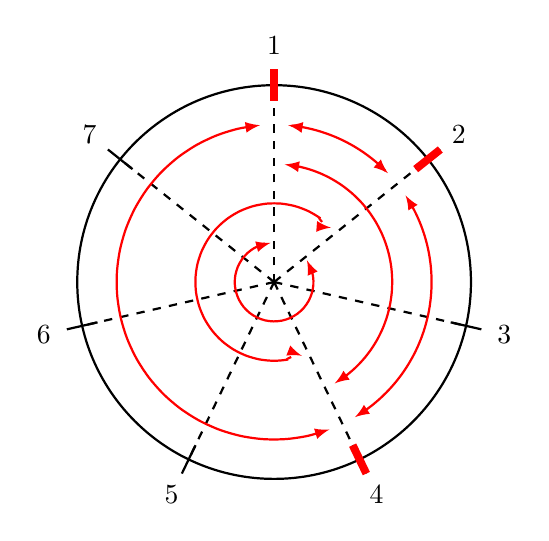
\begin{tikzpicture}
        \def\N{7}
        \draw [thick, black] circle[radius=2.5cm] (0,0);
        \foreach \i in {1,...,\N} {
            \draw [scale=1,domain=2.3:2.7,smooth,variable=\x,black,thick] plot ({\x*sin(360*(\i-1)/\N)},{\x*cos(360*(\i-1)/\N)});
            \draw [black,thick,dashed] (0,0) -- ({2.5*sin(360*(\i-1)/\N)},{2.5*cos(360*(\i-1)/\N)});
            \node[black] at ({3*sin(360*(\i-1)/\N)},{3*cos(360*(\i-1)/\N)}) {$\i$};
        }
        \foreach \i in {0,1,3} {
            \draw [scale=1,domain=2.3:2.7,smooth,variable=\x,red,line width=1mm] plot ({\x*sin(360*\i/\N)},{\x*cos(360*\i/\N)});
        }
        \draw [scale=1,domain=0.1:0.9,smooth,variable=\x,black,thick,>=latex,<->,red] plot ({2*sin(360*\x/\N)},{2*cos(360*\x/\N)}); % 1
        \draw [scale=1,domain=1.1:2.9,smooth,variable=\x,black,thick,>=latex,<->,red] plot ({2*sin(360*\x/\N)},{2*cos(360*\x/\N)}); % 2
        \draw [scale=1,domain=3.1:6.9,smooth,variable=\x,black,thick,>=latex,<->,red] plot ({2*sin(360*\x/\N)},{2*cos(360*\x/\N)}); % 4
        \draw [scale=1,domain=0.1:2.9,smooth,variable=\x,black,thick,>=latex,<->,red] plot ({1.5*sin(360*\x/\N)},{1.5*cos(360*\x/\N)}); % 3
        \draw [scale=1,domain=3.1:7.9,smooth,variable=\x,black,thick,>=latex,<->,red] plot ({1*sin(360*\x/\N)},{1*cos(360*\x/\N)}); % 5
        \draw [scale=1,domain=1.1:6.9,smooth,variable=\x,black,thick,>=latex,<->,red] plot ({0.5*sin(360*\x/\N)},{0.5*cos(360*\x/\N)}); % 6
    \end{tikzpicture}
    \caption{Minimal circular ruler for $N=7$}
    \label{fig:circular-ruler}
\end{figure}

D.Ariananda and G.Leus \todo{ref}


\end{document}
